
\vspace*{-5pt}

\section{Theoretical framework: overview} 
\label{sec:framework}

\begin{figure}[t]
 \vspace{-0.35in}
    \centering
        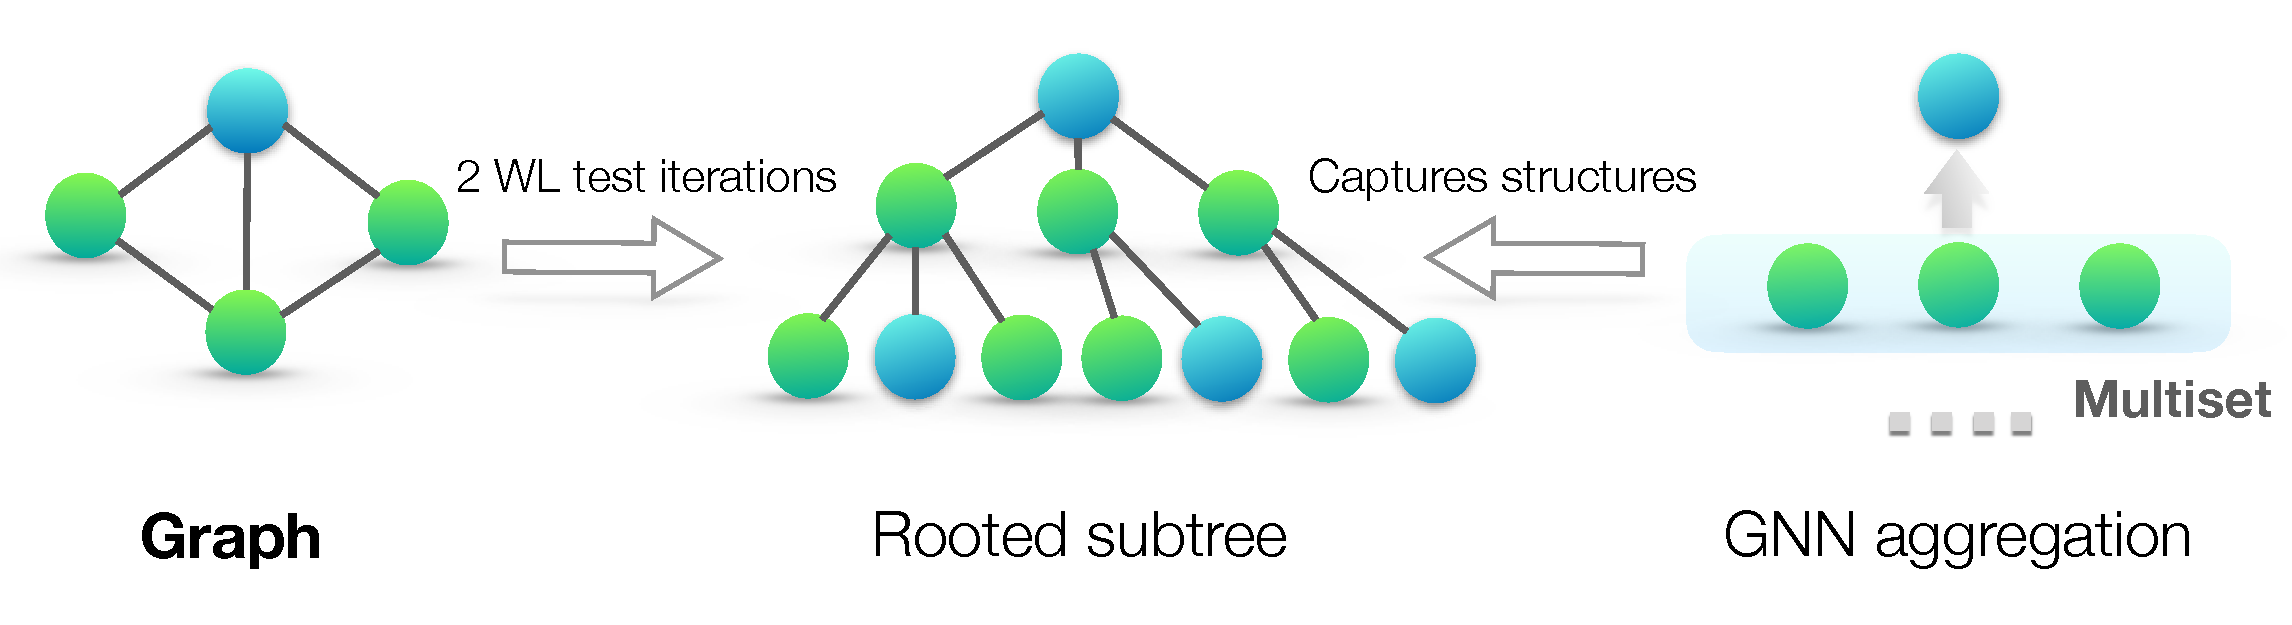
\includegraphics[width=0.9\textwidth]{frame.pdf} \vspace{-0.1in}
    \caption{{\bf An overview of our theoretical framework.} Middle panel: rooted subtree structures (at the blue node) that the WL test uses to distinguish different graphs. Right panel: if a GNN's aggregation function captures the \textit{full multiset} of node neighbors, the GNN can capture the rooted subtrees in a recursive manner and be as powerful as the WL test.}
\label{fig:wl-trees} \vspace{-0.00in}
\end{figure}

We start with an overview of our framework for analyzing the expressive power of GNNs. Figure~\ref{fig:wl-trees} illustrates our idea. A GNN recursively updates each node's feature vector to capture the network structure and features of other nodes around it, \ie, its rooted subtree structures (Figure~\ref{fig:wl-trees}). 
\revise{Throughout the paper, we assume node input  features are from a countable universe. For finite graphs, node feature vectors at deeper layers of any fixed model are also from a countable universe.}
%
For notational simplicity, we can assign each feature vector a unique label in $\{a, b, c \ldots\}$. Then, feature vectors of a set of neighboring nodes form a \emph{multiset} (Figure~\ref{fig:wl-trees}): the same element can appear multiple times since different nodes can have identical feature vectors. 

\begin{definition}[Multiset] \label{def:multiset}
A multiset is a generalized concept of a set that allows multiple instances for its elements. More formally, a multiset is a 2-tuple $X = (S, m)$ where $S$ is the \textit{underlying set} of $X$ that is formed from its \textit{distinct elements}, and $m: S \rightarrow \mathbb{N}_{\geq 1}$ gives the \textit{multiplicity} of the elements. 
\end{definition} 

To study the representational power of a GNN, we analyze when a GNN maps two nodes to the same location in the embedding space. Intuitively, a maximally powerful GNN maps two nodes to the same location \textit{only if} they have identical subtree structures with identical features on the corresponding nodes. Since subtree structures are defined recursively via node neighborhoods (Figure~\ref{fig:wl-trees}), we can reduce our analysis to the question whether a GNN maps two neighborhoods (\ie, two multisets) to the same embedding or representation. A maximally powerful GNN would \textit{never} map two different neighborhoods, \ie, multisets of feature vectors, to the same representation. This means its aggregation scheme must be \textit{injective}. Thus, we abstract a GNN's aggregation scheme as a class of functions over multisets that their neural networks can represent, and analyze whether they are able to represent injective multiset functions. 

Next, we use this reasoning to develop a maximally powerful GNN. In Section \ref{sec:theory}, we study popular GNN variants and see that their aggregation schemes are inherently not injective and thus less powerful, but that they can capture other interesting properties of graphs.